
\section{Overview}
\label{sec:overview}
\sysname is a smartphone-based blood glucose level tracking system that \emph{(i)} non-intrusively collects important external impacting factors and conducts feature engineering, \emph{(ii)} efficiently trains a personalized blood glucose level model via a novel multi-division deep learning framework, and \emph{(iii)} timely reminds users of abnormal blood glucose levels.
\figref{fig:architecture} shows the architecture of \sysname, which consists of three modules.

\begin{figure}[h]
  \centering
  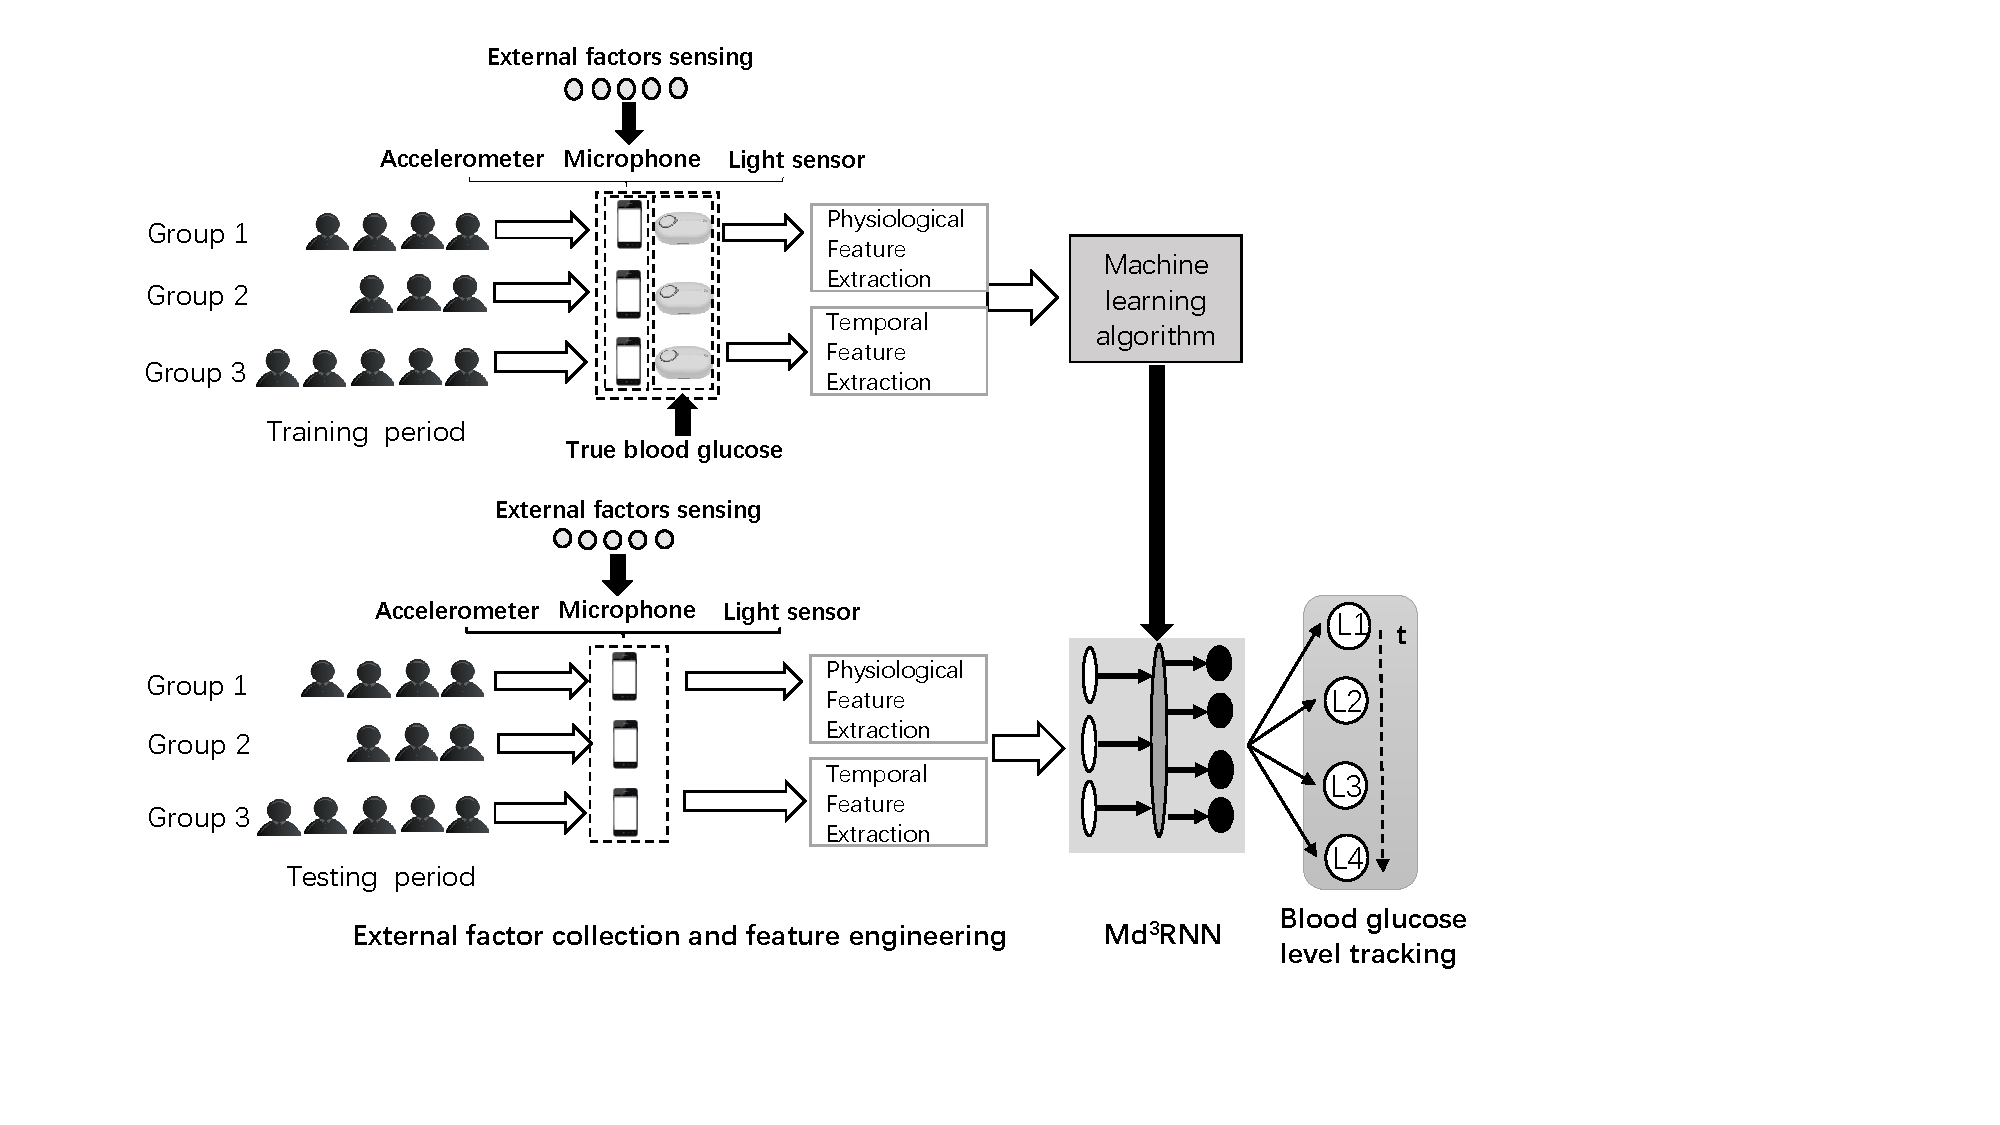
\includegraphics[width=0.85\columnwidth]{./img/System_Arch2.pdf}
  \caption{Architecture of \sysname.}
  \label{fig:architecture}
\end{figure}


The \textbf{external factor collection and feature engineering} module first records external factors that are not only important to infer blood glucose concentration but also convenient to input via smartphones. A user enters meta information (\eg health status, age, weight), and records daily meal, drug and insulin intake.
Meanwhile, \sysname will automatically measures physical activities and sleep quality of the user via embedded sensors (\ie accelerometer, microphone and light sensor). After collecting data from multiple users, \sysname conducts feature engineering from physiological and temporal perspectives, and feeds them into a multi-division deep learning framework: \textbf{\modelname}.
\modelname first learns feature representations from users in the same group (non-diabetic, type I and type II diabetic), and then adopts a deep RNN layer to learn a general blood glucose level model on the dataset of all users.
Finally, it outputs a personalized blood glucose level model for each individual via a personality layer. The personalized inference results of blood glucose level at fine-grained time resolution are eventually shown in the \textbf{blood glucose level tracking} module, reminding the users of the abnormal levels of blood glucose.
In \sysname, we consider 4 blood glucose levels as in \tabref{tab:blood_glucose_levels}.

As shown in \figref{fig:architecture}, the true blood glucose values sampled by CGM are used as labels of model training. The users do not need to wear CGM when they run \sysname in daily life (\ie testing period).

%As such, a user-friendly interface is designed to decompose the input process into multiple menu selections.

\begin{table}[h]
  \centering
  \caption{Normal and abnormal blood glucose levels~\cite{bib:BGWiKi}. The normal blood glucose concentration ranges from 4.4 mmol/L to 6.1 mmol/L. The blood glucose can grow to 7.8 mmol/L after eating. Blood glucose above 7.8 mmol/L for a prolonged period indicates the risk of diabetes mellitus. Blood glucose below 4.4 mmol/L is a sign of hypoglycemia.}
  \label{tab:blood_glucose_levels}
  \begin{tabular}{|c|c|c|}
  \hline
  \textbf{Blood Glucose Value (mmol/L)} & \textbf{Glocose Level} & \textbf{Explanation}                      \\ \hline
  (0, 4.4{]}                            & Level 1                & Low blood glucose (hypoglycemia)         \\ \hline
  (4.4, 6.1{]}                          & Level 2                & Normal level of fasting blood glucose      \\ \hline
  (6.1, 7.8{]}                          & Level 3                & Normal level of postprandial blood glucose \\ \hline
  (7.8, $+\infty$)                      & Level 4                & High blood glucose (hyperglycemia)          \\ \hline
  \end{tabular}
\end{table}


%The framework of \sysname is shown as \figref{fig:architecture}, consisting of four major components.
%The first one is the external factors collection.
%The users are required to enter their basic information into application, including of the age, the gender, the diabetes type and the year of diagnosis.

%After a user measures his/her blood glucose by a CGM, the records of the blood glucose along with the outer contextual factors occurred during the measurement are uploaded to an individual database automatically.
%Afterwards, a RNN model is trained based on the dataset to establish the relationships between the outer contextual factors and the corresponding blood glucose level.
%It then is fed into the user's smartphone.
%When the user does not wear the CGM, \sysname detects the outer contextual factors with embedded sensors in the smartphones, and infers the current blood glucose level based on the trained model.
%Once \sysname detects the abnormal points of blood glucose ( \ie in a \emph{high} or \emph{low} blood glucose level ), it reminds the user to measure the blood glucose by a clinical CGM for a further control.

%The extraction mechanisms of outer contextual factors are detailed as follows.
%
%\emph{Physical activity}:
%\sysname leverages the accelerometer to detect the user's activities by the approaches in \cite{bayat2014study}, as well as the corresponding time costs.
%\sysname then measures the calorie of user's physical consumption.
%
%\emph{Food intake}:
%\sysname measures the food's effect on a person's blood glucose level based on the glycemic index.
%
%\emph{Clinical drug intake}:
%\sysname records the name and amount of the drug that user eat.
%
%\emph{Time}:
%\sysname invokes the timer embedded in the smartphone to record the time.
%
%\emph{Sleep quality}:
%\sysname measures the user's sleep by the approach in \cite{gu2014intelligent}.
